\documentclass{article}
\usepackage[utf8]{inputenc}
\usepackage{amsmath}
\usepackage{graphicx}
\usepackage{xcolor}
\usepackage{natbib}
\bibliographystyle{plainnat}
\title{Our Spatial Paper}
\author{Your Name}
\date{\today}

\begin{document}

\maketitle

\begin{abstract}
    Please be concise.
\end{abstract}

\section{Project Plan}
\begin{itemize}
    \item Idea Formation and Lit Review  Jan 13-17  [together ]
    \item Theory - Coming up with a Model/Try to meet with Esteban to get feedback? Jan 20-22 [together]
    \item Theory - Solving the Model Jan 23-24 [Key Person = Henrique]
    \item Coding (data, estimation, counterfactual, and results) - Jan 27 - Jan 31  [Key Person = ]
    \begin{itemize}
        \item Inputs are fairly divisible
        \item Outputs are less divisible
        \item Writing -  Feb 4 - 7  (KeyPerson)
   \end{itemize}
\end{itemize}
\section{Meeting Notes}
\begin{enumerate}
    \item  Could have teams of (2) for various things. 
    \item There are some tasks that are independent. 
    \item Decide to break stuff up once we actually have an idea.
    \item Henrique: Likes Lit Review / Idea Formation / Likes Writing [let us simplify model if possible]. Prefers the equilibrium part of coding to the early / data cleaning part Less good at Geodata.  Very good at polishing and visual details. 
    \item Jeffrey: Likes Coding / Likes Writing
    \item Yulia: Interested in counterfactuals part of coding. Curious about theory. Experience about writing / likes writing. 
\end{enumerate}

\subsection{ for next meeting, Jan 17 }
\begin{enumerate}
    \item Read model / counterfactuals of Monte et al in detail enough 
    \item In the Esteban choose your model 
    \item Map Monte et al to Esteban's choose your model. 
    \item Look at Jeffrey's ideas. 
\end{enumerate}



\subsection{During next meeting}
\begin{enumerate}
    \item pick idea
    \item assign data 
\end{enumerate}


\section{Introduction}
\label{sec:intro}
Your introduction here.

\section{Background and Diagnostic}
Prompt:Why is the question or policy you want to examine
important? Why is a quantitative spatial model the right tool to answer the question?
Are there any particular features of the policy/economic environment that are impor-
tant for the analysis? Feel free to focus on one or a few aspects that you want to study
in depth and identify the underlying mechanisms, which will inform you about the key
elements to be included in your model.
\subsection{Brainstorming }

\subsubsection{Idea 1: Self-driving cars}
The original invention of the internal combustion engine
radically transformed rents, population density, and the distribution of economic activity. 

The rise of self-driving cars is likely to have a similar transformative effect on the spatial distribution of economic activity.
Waymo currently operates self-driving cars in Phoenix, Arizona, Los Angeles, CA, and San Francisco, CA.



Our first counterfactual will thus be the introduction of self-driving cars in these three counties, which collectively comprise 
XYZ share of the US population, and  \$PQR share of GDP.

Our second counterfactual will be to introduce self-driving in all counties.

Our third counterfactual, which is most policy-relevant, will be the introduction of self-driving in the top [XXX\%] of counties by some measure of regulatory friendliness.
 This will allow us to study a setting where a sizable chunk of the US economy has self-driving, and the rest doesn't. This is inspired by the real-world heterogeneity in regulations, compare, e.g. California and Arizona to, e.g., New York.
 
 his will let us speak to distributional effects (welfare, rents, population) of heterogeneity in self-driving car regulation.

\textcolor{red}{Fundamentally, this amounts to what do you mean by ``introduction''? 100\% use of car trips become this?
does any walking or biking or public transit substitute towards this?}

With American Time Use Data, which not only reports how much time people spend on various activities, but how much they like or dislike them, we can microfound the cost of commuting (maybe there is another paper we can take this from, instead, too), and building on YYY paper, which compares the cost of commuting by public transit vs. cars, 
we can back out how the primitives of commuting costs change in XYZ locations.



Important things here:
\begin{enumerate}
    \item Isn't it obvious that a decline in commuting costs would lead people to spread out? Does it matter that it's self-driving cars causing this decline? 

    \item Do you model the choice of how to commute, or just reduced-form things?
\item Just reducing $\kappa_{ni}$ for these places seems a little lazy
\item Might the interesting angle to be quantify how places that are slow-to-allow self driving cars ``fall behind'', in some sense, those which are faster to allow it? 
\item Do we think that (me using a self driving car) has a positive externality on other people?
\item Any pecuniary costs in the counterfactual (e.g. I have to buy a self driving car), or just the commuting costs?
\item Will self-driving have a homogeneous effect on all $\kappa_{ni}$? Probably should only apply to certain node-pairs where people are driving.
\end{enumerate}

\subsubsection{Idea 2: Incorporating car ownership}
Who owns cars, where, and why?

Is the cost of car ownership incorporated into the indifference conditions of these spatial models: maybe chicago isn't actually much cheaper than e.g. nyc once you add a car payment to your rent [which many more people seem to have / beed in Chicago] 


Kind of tricky. Need some heterogeneity to endogenize this choice which already complicates things.

Could have $\kappa^{car}_{ni}$ <
$\kappa^{no \ car}_{ni} $ and people choose to pay a fixed cost for a car or not. 
Then, who gets a car vs. who doesn't? 
People who have higher preference for space, $\alpha_i$

Could just have a owning a car as an effective decline in wage (rather than an asset).
If we wanted to really get fancy, we could have heterogeneous commuting costs, i.e. weight or power $\kappa_{ni}$ by something. 


\subsubsection{Idea 3: }
I wonder if Amazon has impacted car ownership through making it easier to just have a bunch of stuff delivered. 
And this in turn reduces congestion? Seems second-order, maybe not.

\subsubsection{Idea 4: Crime $\rightarrow$ Commuting}
My intuition is that, all else equal, people take public transit less in a city if crime ( LA buses, for example, Chicago red line, more recently, NY Subway).

Does this impose a quantitatively important externality on commuting costs, by shifting people to cars?

In a complete paper, we would endogenize crime, by also examining how available commuting influences crime, as well. 

\subsubsection{Idea 5: Weather, Commuting Costs, and Climate Change}
Climate change may have distributional consequences on commuting costs:
places like Florida may see more precipitation. Places like Chicago may see fewer snowy days [citation needed]
\subsubsection{Idea 6: Zoning in car cities vs walkable cities}

\subsubsection{Idea 7: Distributional Efects of parking requirements}
Maybe minimum parking requirements in business areas let fewer people live in the city, but lowers commute times for the people that do commute.
\subsubsection{Idea 8: Car safety and commuting}
\begin{figure}
    \centering
    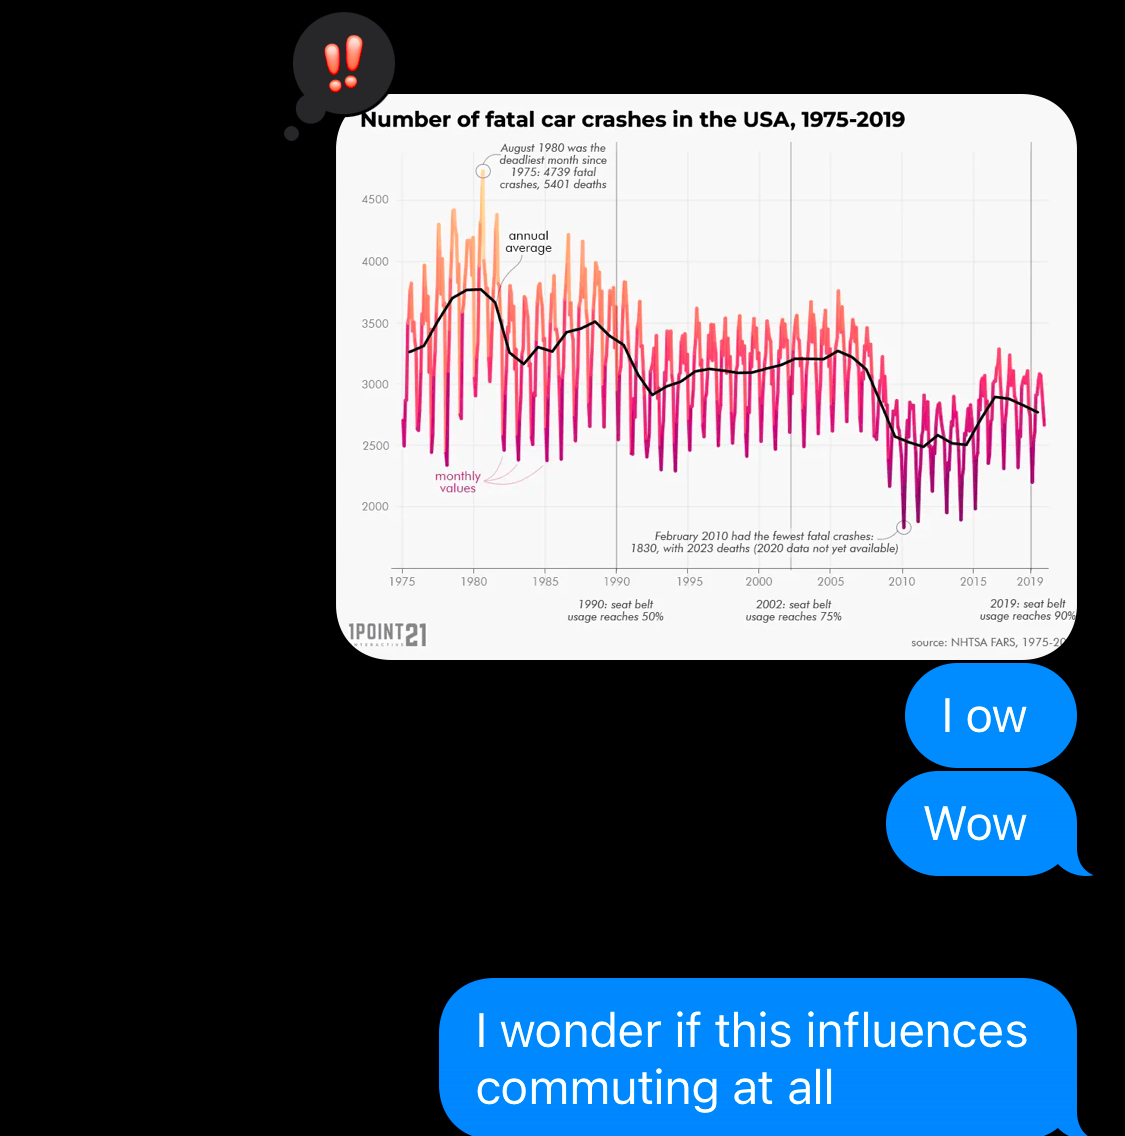
\includegraphics[width=0.5\textwidth]{img/cardeaths.jpeg}
    \caption{Deaths per capita in the US from car accidents.}
    \label{fig:car_deaths}
\end{figure}
\section{Model}

\subsection{Jeff's notes on Monte et al model}
\begin{enumerate}
\item It's a bit weird to have this `E[]' component. WTF. Are we treating it as random which place they commute to? Yes.
\item Amenities are our idiosyncratic term and are paramterized by $b_{ni\omega}$, that they can differ by person and where they live / work. Or better, put: they each get $N^2$ shocks.
\item Goods - standard
\item Closing the land market: landlords own everything.
\item People's utility is just in land. So there's no housing being created people just eat $C$ and $H$.
\item  When can we use exact hat algebra for counterfactuals? (see Eqn. 24)
\end{enumerate}

Write down the model that directly speaks to the mechanisms you identified
in the previous step. You need to specify all the building blocks and solve for the
equilibrium (equilibria). Please be clear and concise, and feel free to leave tedious
derivations in the appendix or cite any relevant derivations you want to lift from
existing papers.
You are encouraged to tweak or simplify an existing model, like the one in Monte et
al. (2018). If you want to be more creative, feel free to select components from the
“menu of quantitative spatial models” in Section 2 of Redding and Rossi-Hansberg
(2017). When tweaking an existing model or building a model of your own, make
sure you include only the necessary elements related to your proposed mechanisms.
Importantly, please be aware of the time and feasibility constraints when specifying
your model.

\section{Data and Estimation}
\label{sec:data}
Describe the data you use to estimate the model. What
variables do you need? How do you access them? How do you plan to estimate the
model? For parameters that you will calibrate, justify your choices. For parameters
that you will estimate, explain your strategy.

\section{Counterfactual}
\textbf{It seems like this is the area for creativity. We can keep the model itself as in Monte}
\label{sec:counterfactual}
Carefully describe the counterfac-
tual exercise (i.e., a policy that you want to evaluate) you want to examine. What is your plan for implementing it? Are you going to fully invert the model to back out
fundamentals? Are you going to use exact hat algebra to solve the model in changes?
For the purpose of this problem set, you can restrict your attention to policies that
are local in nature (i.e., policies that target a specific county or a set of counties
independently of others). If you are interested in a non-local policy (i.e. a policy like a
construction of interstate highways that affect many counties similtaneously), you do
not need to compute changes in fundamentals with high level of precision (e.g., changes
in commuting costs in each county), a rough approximation will suffice

\section{Appendix}
Painful proofs go here.

\bibliography{references}

\end{document}